\thispagestyle{toancuabinone}
\pagestyle{toancuabi}
\everymath{\color{toancuabi}}
\blfootnote{$^1$\color{toancuabi}Đại học Thăng Long.}
\graphicspath{{../toancuabi/pic1/}}
\begingroup
\AddToShipoutPicture*{\put(0,616){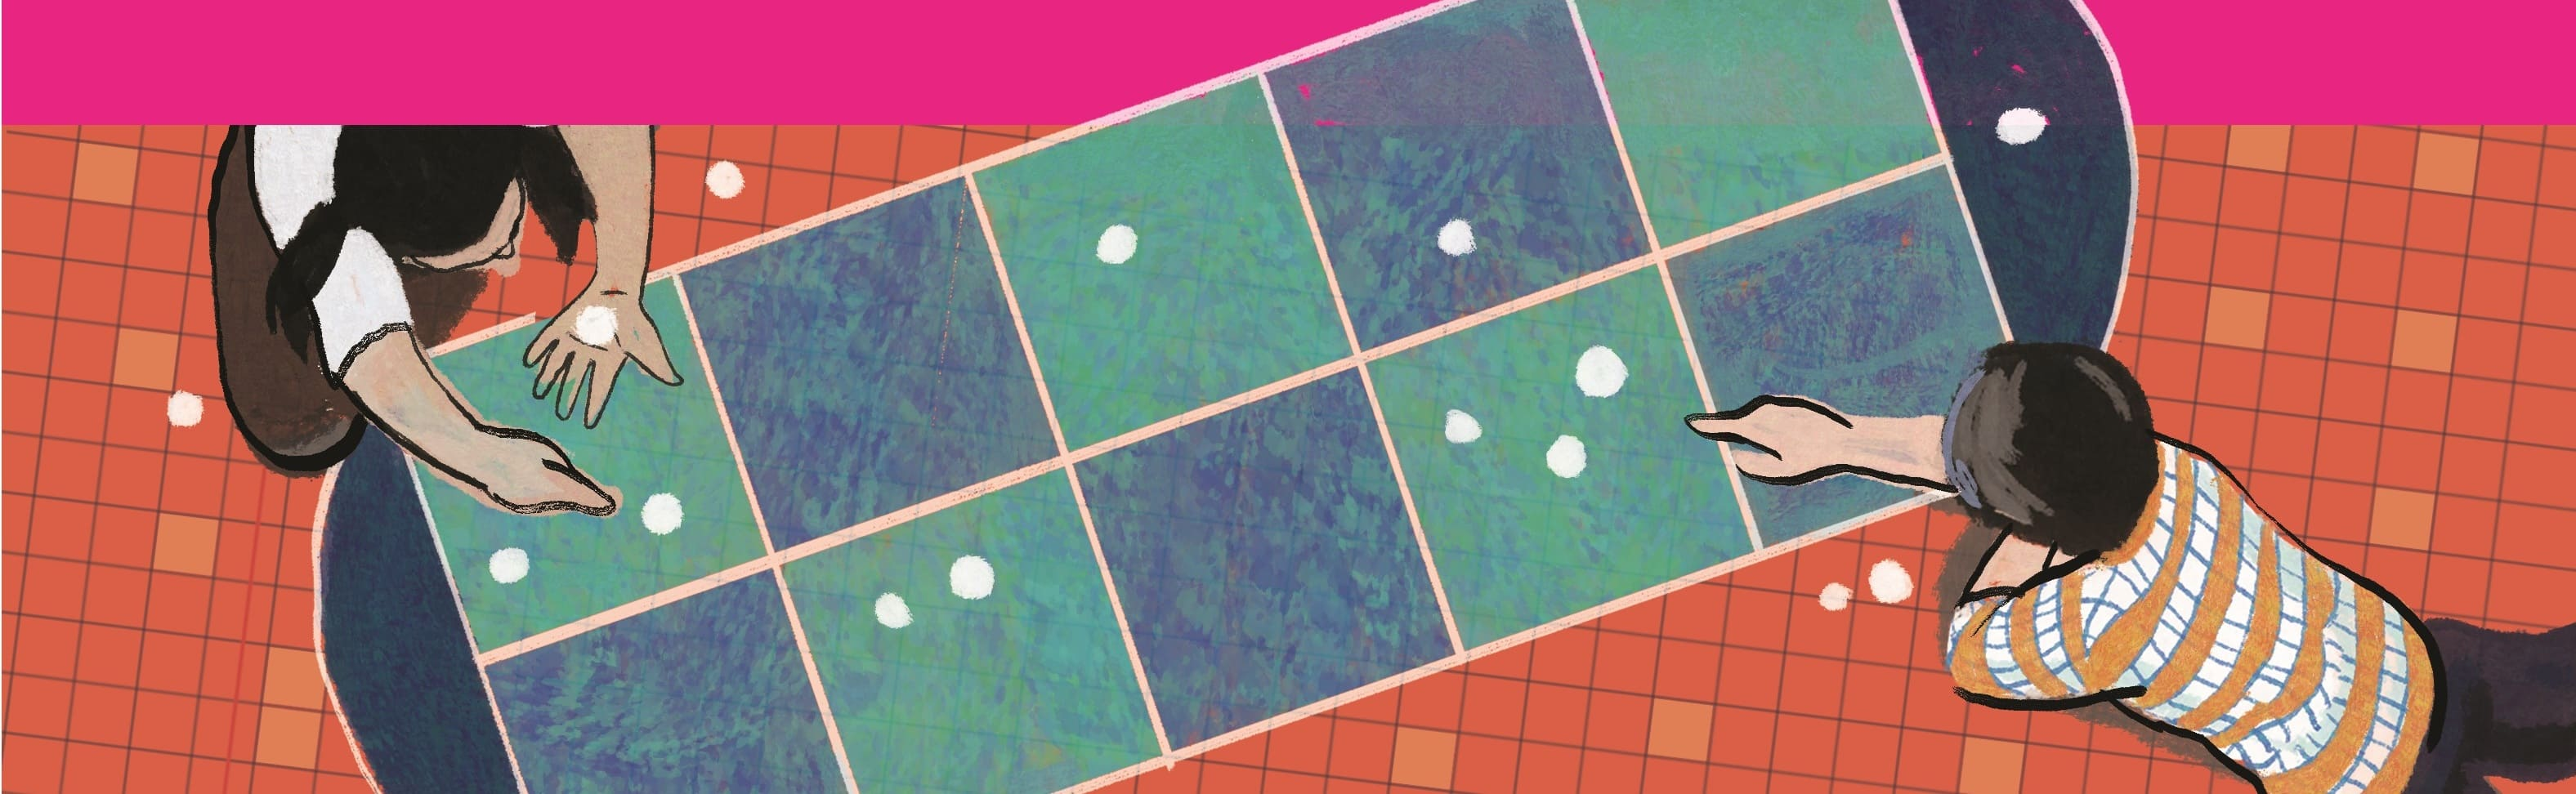
\includegraphics[width=19.3cm]{../bannertoancuabi}}}  
\AddToShipoutPicture*{\put(104,525){
\includegraphics[scale=1]{../tieude1.pdf}}} 
\centering
\endgroup
\vspace*{185pt}


\begin{multicols}{2}
	Trong phần $1$ của bài viết, các em đã được giới thiệu về số tượng hình của người Ai Cập cổ và cách ghi số của người La Mã dựa trên một số chữ cái trong bảng chữ cái. Trong phần $2$ này, chúng ta sẽ cùng tìm hiểu về số Babylon, số Maya và số Trung Hoa cổ.
	\vskip 0.1cm
	\textbf{\color{toancuabi}Số Babylon}
	\vskip 0.1cm
	Người Babylon, sống vào khoảng $5000$ năm trước ở vùng đất Lưỡng Hà (một khu vực ở phía Tây của  Châu Á). Họ đã tạo ra những công cụ tính toán thiên văn, hình học đáng kinh ngạc và họ đã phát minh ra bàn tính.
		\begin{figure}[H]
		\centering
		\vspace*{-5pt}
		\captionsetup{labelformat= empty, justification=centering}
		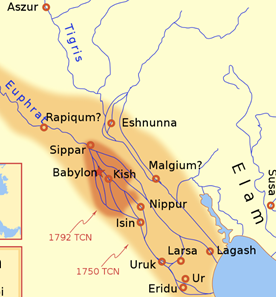
\includegraphics[width=1\linewidth]{17.1}
		\vspace*{-15pt}
	\end{figure}
	Để ghi số, ban đầu người Babylon chỉ sử dụng hai ký hiệu 
	\begin{table}[H]
		\vspace*{-5pt}
		\centering
		\begin{tabular}{|c|c|}
			\hline
			& \\[-2.5ex]
			
\includegraphics[scale=0.7]{15}&$1$\\
			\hline
			& \\[-2.5ex]
			
\includegraphics[scale=0.65]{16}&$10$\\
			\hline
		\end{tabular}
		\vspace*{-5pt}
	\end{table}
	để viết số từ $1$ tới $60$, chẳng hạn số $7$ là  
\includegraphics[scale=0.7]{17}, số $27$ là  
\includegraphics[scale=0.7]{16}
\includegraphics[scale=0.7]{16}
\includegraphics[scale=0.7]{17}. 	 
	\vskip 0.1cm
	Những ký hiệu này được sử dụng tương tự như những chữ số La Mã (bằng cách cộng các ký hiệu xuất hiện trong số được biểu diễn). Số 
\includegraphics[scale=0.7]{18} được viết bởi $2$ ký hiệu 
\includegraphics[scale=0.7]{16} để biểu diễn $2$ chục, và $7$ ký hiệu 
\includegraphics[scale=0.7]{15}  cho $7$ đơn vị. Do vậy 
\includegraphics[scale=0.7]{18}  $=27$.
	\vskip 0.1cm
	Sau đó, một ký hiệu mới được sử dụng để biểu diễn chữ số $0$, đó là:
	
\includegraphics[scale=0.65]{15.1}
	\vskip 0.1cm
	Để viết những số từ $60$ trở đi, người Babylon xếp các ký hiệu theo các nhóm. Điều này giống như ngày nay các bạn viết $159$ bằng cách viết chữ số $1$ đầu tiên ở hàng trăm, chữ số $5$ tiếp theo ở hàng chục và cuối cùng là chữ số $9$ ở hàng đơn vị. Như vậy $159 = 1 \times 100+ 5 \times 10+ 9$.
	\vskip 0.1cm
	Để viết số $63$, người Babylon viết ký hiệu  
\includegraphics[scale=0.7]{15}  ở hàng $60$ và ba ký hiệu 
\includegraphics[scale=0.7]{15}  ở hàng đơn vị và để khoảng trống để phân biệt hai nhóm.
	\vskip 0.1cm
	Như vậy, 
\includegraphics[scale=0.7]{16.1}$=63$. Trong cách viết này, ta thấy có $4$ ký hiệu 
\includegraphics[scale=0.7]{15}   nhưng ký hiệu đầu tiên được viết tách biệt so với $3$ ký hiệu còn lại để biểu diễn $1$ lần $60$ tức $60$, $3$ ký hiệu còn lại biểu diễn số $3$, và như vậy ta có số $60+3 =63$.
	\vskip 0.1cm
	Điều này giống như chúng ta viết chữ số $1$ ở hàng chục và chữ số $1$ ở hàng đơn vị để biểu diễn số $11$: nó có nghĩa là $1$ chục và $1$ đơn vị. Trong  cách ghi số  Babylon cổ, nó có nghĩa là $1$ lần $60$  và $1$.
	\begin{figure}[H]
		\centering
		\vspace*{-5pt}
		\captionsetup{labelformat= empty, justification=centering}
		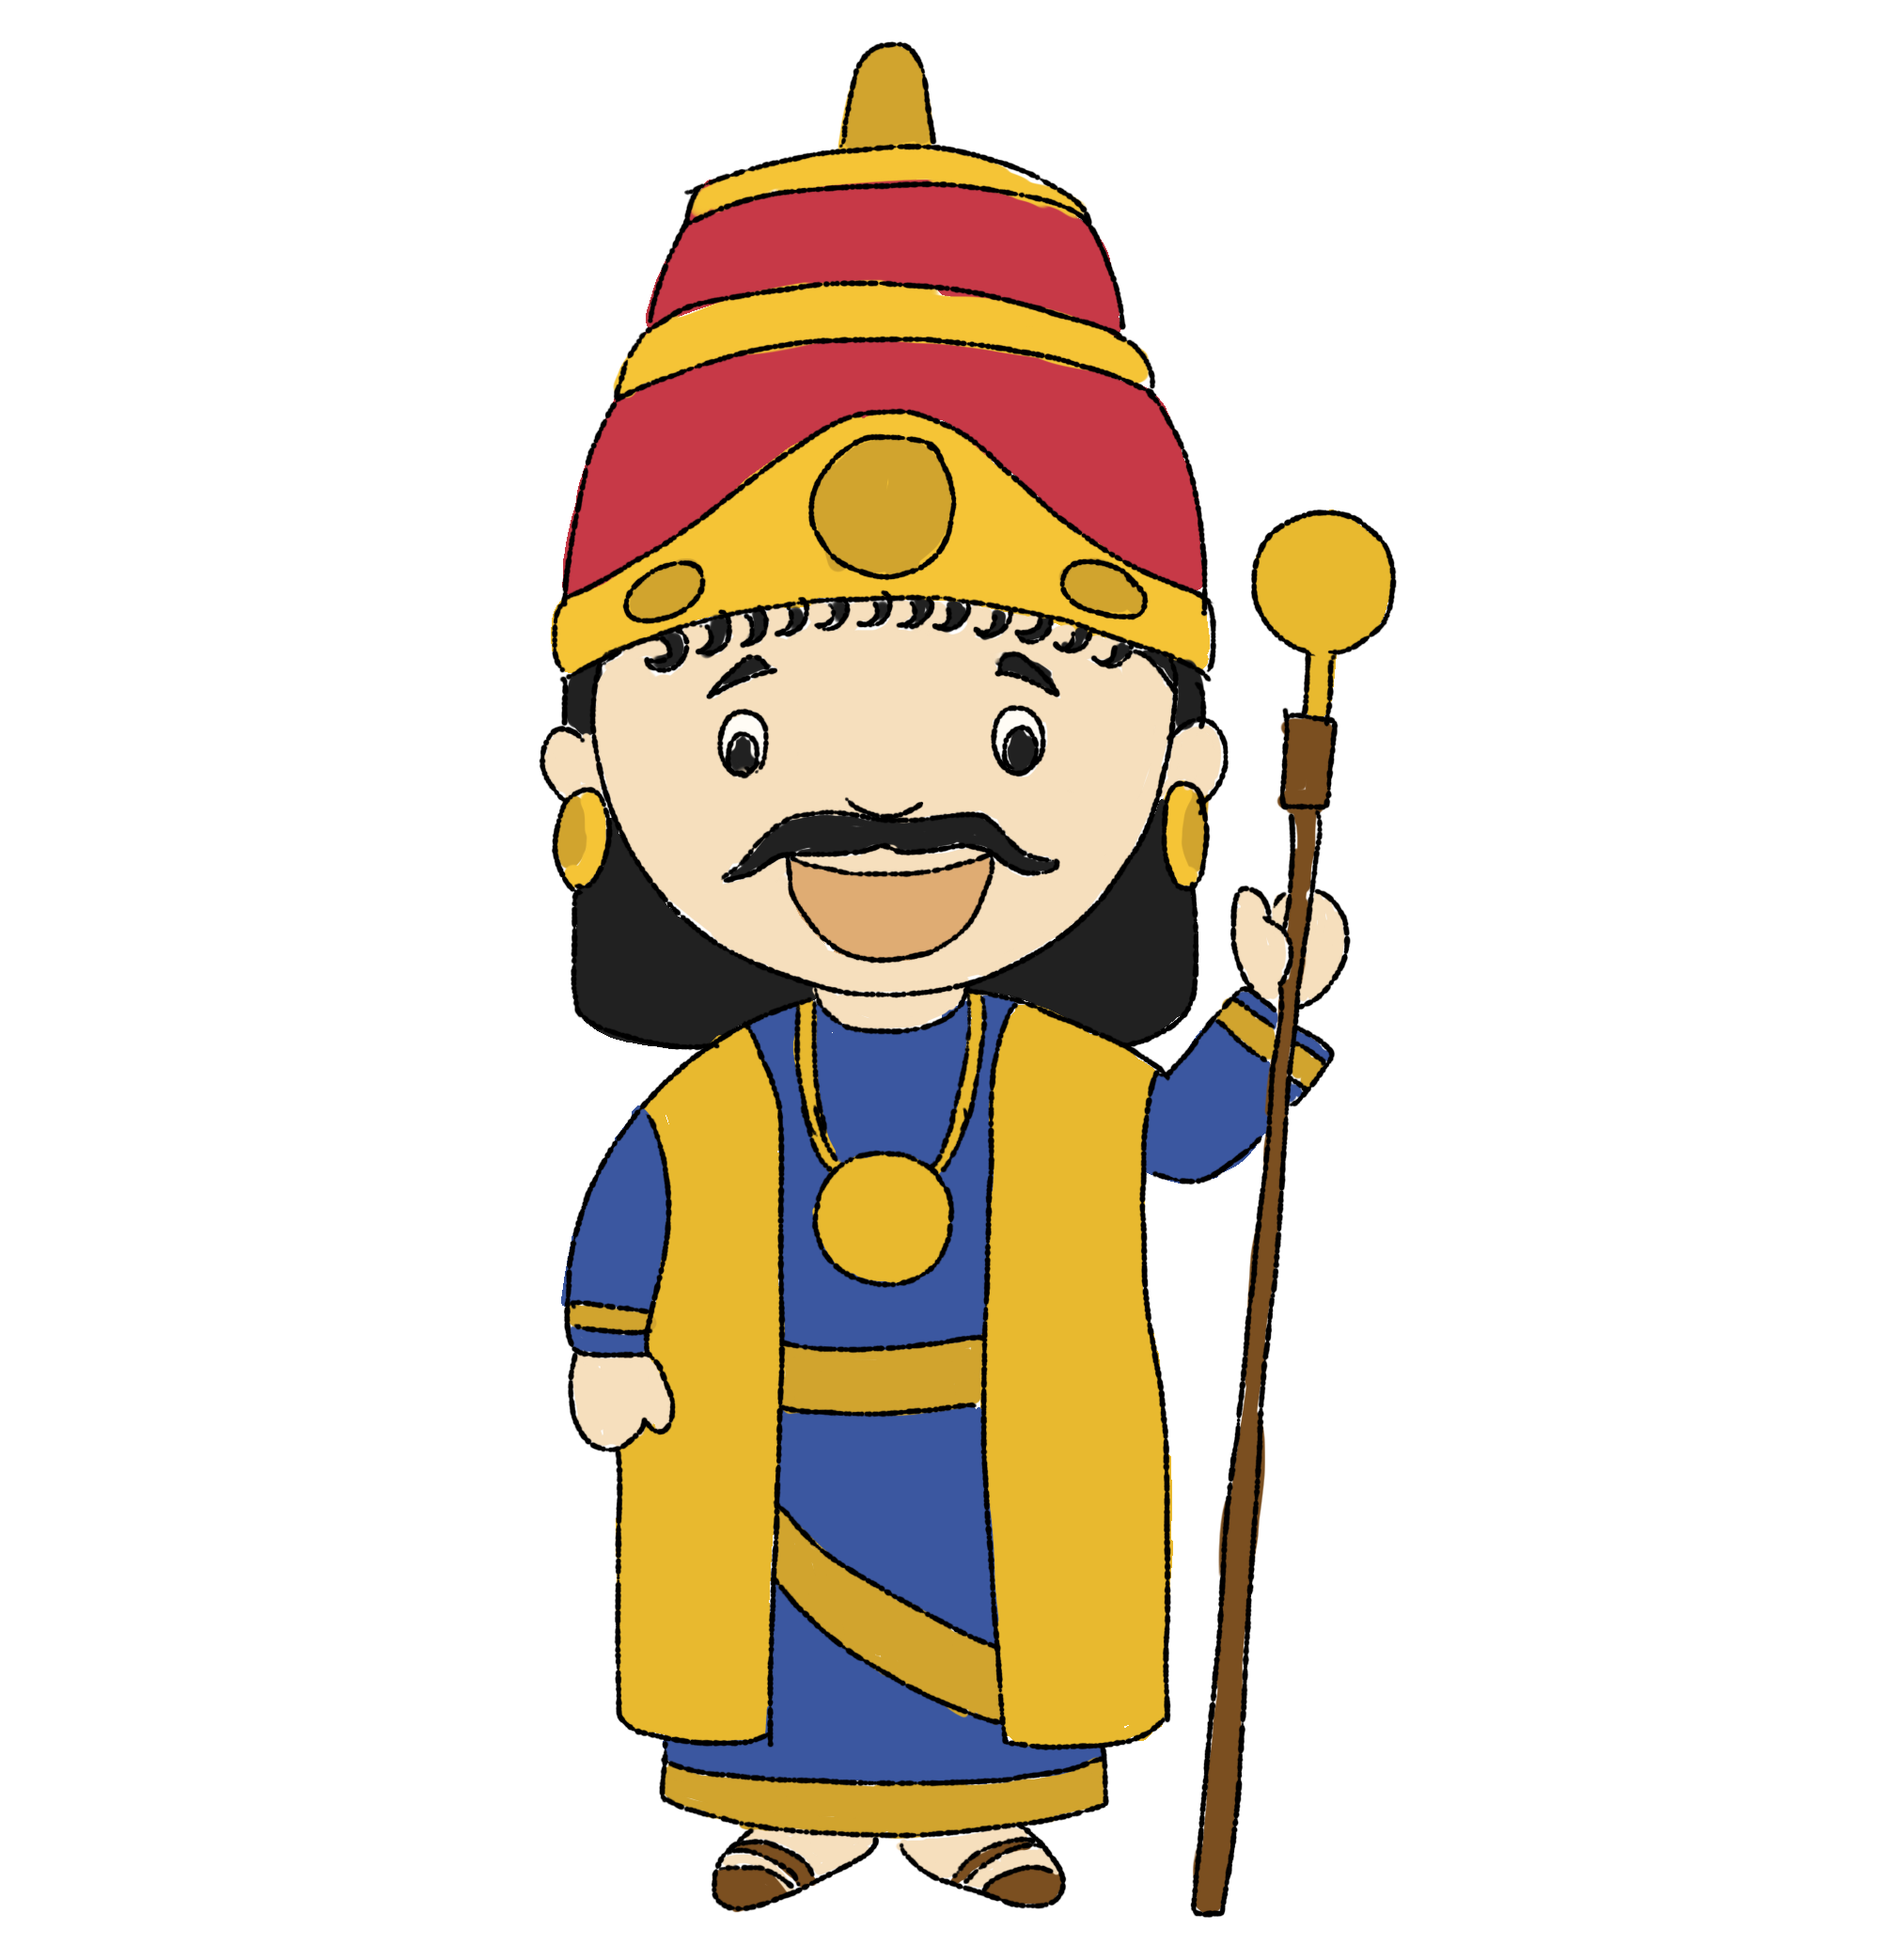
\includegraphics[width=0.85\linewidth]{20.12-pi.2}
		\vspace*{-15pt}
	\end{figure}
	Để hiểu rõ hơn, ta hãy viết số chín mươi ba theo cách ghi số hiện nay. Việc này thật dễ dàng phải không? Tuy nhiên, để hiểu cách viết của người Babylon, ta sẽ thực hiện theo cách như sau: do chúng ta sử dụng hệ cơ số $10$, ta chia chín mươi ba cho $10$ được thương là $9$, nên ta viết $9$ vào hàng chục:
	\begin{figure}[H]
		\centering
		\vspace*{-5pt}
		\captionsetup{labelformat= empty, justification=centering}
		\begin{tikzpicture}[xscale=1.5,yscale=1.2,color=toancuabi]
			\draw (0,0) grid (3,1);
			\draw (1.5,0.5) node {$9$};
			\draw (0.5,1.05) node[above] {$\scriptstyle\times(10\times10)$};
			\draw (1.5,1.1) node[above] {$\scriptstyle\times10$};
			\draw (2.5,1.1) node[above] {$\scriptstyle\times1$};
		\end{tikzpicture}
		\vspace*{-10pt}
	\end{figure}
	Phép chia đó có số dư $3$ nên ta viết $3$ vào hàng đơn vị:
	\begin{figure}[H]
		\centering
		\vspace*{-5pt}
		\captionsetup{labelformat= empty, justification=centering}
		\begin{tikzpicture}[xscale=1.5,yscale=1.2,color=toancuabi]
			\draw (0,0) grid (3,1);
			\draw (1.5,0.5) node {$9$};
			\draw (2.5,0.5) node {$3$};
			\draw (0.5,1.05) node[above] {$\scriptstyle\times(10\times10)$};
			\draw (1.5,1.1) node[above] {$\scriptstyle\times10$};
			\draw (2.5,1.1) node[above] {$\scriptstyle\times1$};
		\end{tikzpicture}
		\vspace*{-10pt}
	\end{figure}
	Vậy là ta viết: $93$.
	\vskip 0.1cm
	Số chín mươi ba được viết như thế nào với số Babylon?
	\vskip 0.1cm
	Do cách ghi số Babylon sử dụng hệ cơ số $60$, ta chia $93$ cho $60$ được thương là $1$ nên ta viết $1$ ở hàng $60$.
	\begin{figure}[H]
		\centering
		\vspace*{-5pt}
		\captionsetup{labelformat= empty, justification=centering}
		\begin{tikzpicture}[xscale=1.5,yscale=1.2,color=toancuabi]
			\draw (0,0) grid (3,1);
			\node[inner sep=0pt] (mouse) at (1.5,0.5){
\includegraphics[scale=1]{27a.png}};
			\draw (0.5,1.05) node[above] {$\scriptstyle\times(60\times60)$};
			\draw (1.5,1.1) node[above] {$\scriptstyle\times60$};
			\draw (2.5,1.1) node[above] {$\scriptstyle\times1$};
		\end{tikzpicture}
		\vspace*{-10pt}
	\end{figure}
	Phép chia có số dư là $33$, nên ta sẽ viết $33$ ở hàng đơn vị. Số $33$ được biểu diễn bởi $3$ ký tự mười cộng với $3$. Nên ta đặt $3$ ký tự 
\includegraphics[scale=0.65]{16} và $3$ ký tự 
\includegraphics[scale=0.65]{15} vào hàng đơn vị như sau:
	\begin{figure}[H]
		\centering
		\vspace*{-5pt}
		\captionsetup{labelformat= empty, justification=centering}
		\begin{tikzpicture}[xscale=1.5,yscale=1.2,color=toancuabi]
			\draw (0,0) grid (3,1);
			\node[inner sep=0pt] (mouse) at (1.5,0.5){
\includegraphics[scale=1]{27a.png}};
			\node[inner sep=0pt] (mouse) at (2.5,0.5){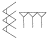
\includegraphics[scale=1]{22a.png}};
			\draw (0.5,1.05) node[above] {$\scriptstyle\times(60\times60)$};
			\draw (1.5,1.1) node[above] {$\scriptstyle\times60$};
			\draw (2.5,1.1) node[above] {$\scriptstyle\times1$};
		\end{tikzpicture}
		\vspace*{-10pt}
	\end{figure}
	Vậy 
\includegraphics[scale=0.9]{23}  $= 93$.
	\vskip 0.1cm
	Tiếp theo, chúng ta hãy thử viết số lớn hơn. Chúng ta hãy cùng viết số $3604$ bằng các chữ số Babylon nhé. Số $3604$ lớn hơn $60\times 60=3600$, nên ta cần biểu diễn số này từ hàng thứ ba tính từ hàng đơn vị. Ta chia số $3604$ cho $3600$ được thương là $1$ nên ta viết ký hiệu 
\includegraphics[scale=0.7]{15}  vào hàng $60\times60$
	\begin{figure}[H]
		\centering
		\vspace*{-5pt}
		\captionsetup{labelformat= empty, justification=centering}
		\begin{tikzpicture}[xscale=1.5,yscale=1.2,color=toancuabi]
			\draw (0,0) grid (3,1);
			\node[inner sep=0pt] (mouse) at (0.5,0.5){
\includegraphics[scale=1]{27a.png}};
			\draw (0.5,1.05) node[above] {$\scriptstyle\times(60\times60)$};
			\draw (1.5,1.1) node[above] {$\scriptstyle\times60$};
			\draw (2.5,1.1) node[above] {$\scriptstyle\times1$};
		\end{tikzpicture}
		\vspace*{-10pt}
	\end{figure}
	Số dư của phép chia là $4$ nhỏ hơn $60$ nên ta viết ký hiệu 
\includegraphics[scale=0.6]{15.1} vào hàng $60$, và $4$ ký hiệu 
\includegraphics[scale=0.7]{15} vào hàng đơn vị. 
	\begin{figure}[H]
		\centering
		\vspace*{-5pt}
		\captionsetup{labelformat= empty, justification=centering}
		\begin{tikzpicture}[xscale=1.5,yscale=1.2,color=toancuabi]
			\draw (0,0) grid (3,1);
			\node[inner sep=0pt] (mouse) at (0.5,0.5){
\includegraphics[scale=1]{27a.png}};
			\node[inner sep=0pt] (mouse) at (1.5,0.5){
\includegraphics[scale=1]{27b.png}};
			\node[inner sep=0pt] (mouse) at (2.5,0.5){
\includegraphics[scale=1]{27c.png}};
			\draw (0.5,1.05) node[above] {$\scriptstyle\times(60\times60)$};
			\draw (1.5,1.1) node[above] {$\scriptstyle\times60$};
			\draw (2.5,1.1) node[above] {$\scriptstyle\times1$};
		\end{tikzpicture}
		\vspace*{-10pt}
	\end{figure}
	Vậy, số $3604$ được người Babylon viết như sau:
	\begin{figure}[H]
		\centering
%		\vspace*{-5pt}
		\captionsetup{labelformat= empty, justification=centering}
		
\includegraphics[width=0.35\linewidth]{27}
		%	\caption{\textit{\color{toancuabi}Hình $1$.}}
		\vspace*{-10pt}
	\end{figure}
	Cách ghi số của người Ai Cập cổ, người La Mã hay chúng ta ngày nay dùng cơ số $10$ còn cách ghi số của người Babylon sử dụng cơ số $60$. Do số $60$ chia hết cho nhiều số: $1,2,3,4,5,6, 10, 12, 15, 20,30$ và $60$, nên việc chia các đại lượng được thực hiện dễ dàng hơn, ít phải dùng đến các phân số. Việc sử dụng đơn vị thời gian: $1$ phút $= 60$ giây, $1$ giờ $= 60$ phút ngày nay là một ảnh hưởng của số Babylon đấy.
	\vskip 0.1cm
	\textbf{\color{toancuabi}Số Maya}
	\vskip 0.1cm
	\begin{figure}[H]
		\centering
		\vspace*{-10pt}
		\captionsetup{labelformat= empty, justification=centering}
		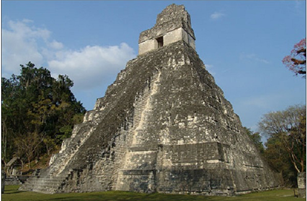
\includegraphics[width=1\linewidth]{28}
		\caption{\textit{\color{toancuabi}Kim tự tháp Tikal của người Maya.}}
		\vspace*{-10pt}
	\end{figure}
	Người Maya  được cho là đã xuất hiện từ rất xa xưa. Họ đã xây dựng hệ thống lịch chính xác và toán học của họ là đại diện tiêu biểu cho toán học của dân cư ở châu Mỹ thời cổ đại.
	\vskip 0.1cm
	Nói về cách ghi số,  người Maya dùng hệ cơ số $20$, gồm $3$ ký hiệu 
\includegraphics[scale=0.7]{29},  
\includegraphics[scale=0.7]{30}, 
\includegraphics[scale=0.7]{31}  ứng với $0,1, 5$ và biểu diễn số theo chiều dọc. Chữ số ở hàng cao hơn được viết phía trên, chữ số ở hàng thấp hơn được viết phía dưới. Điều này tương tự cách chúng ta viết số ngày nay: ta đặt chữ số ở hàng cao hơn bên trái còn chữ số ở hàng thấp hơn bên phải. 
	\begin{table}[H]
		\vspace*{-5pt}
		\centering
		\setlength{\tabcolsep}{4.5pt}
		\renewcommand{\arraystretch}{1.3}
		\begin{tabular}{|l|l|}
			\hline
			$10^3 = 10\!\times\! 10 \!\times\! 10 =1000$& hàng nghìn\\
			\hline
			$10^2 = 10\!\times\! 10 =100$& hàng trăm\\
			\hline
			$10^1 = 10$& hàng chục\\
			\hline
			$10^0 = 1$& hàng đơn vị\\
			\hline
		\end{tabular}
%		\vspace*{-5pt}
	\end{table}
	Do sử dụng hệ cơ số $20$,  số Maya được biểu diễn trong phần bên phải của bảng trong Hình $3$ chính là số  $1\times 8000+ 0\times 400+ 10\times20+ 7\times1= 8207$. Bởi vì, ta  thấy  
\includegraphics[scale=0.3]{33},  
\includegraphics[scale=0.3]{34},  
\includegraphics[scale=0.3]{35}, 
\includegraphics[scale=0.3]{36}  ứng với $1, 0, 10, 7$  lần lượt ở các hàng $8000$, $400$, $20$ và đơn vị. Chú ý rằng, trong một hàng, chữ số có giá trị cao hơn lại được viết phía dưới chữ số có giá trị thấp hơn, chẳng hạn  
\includegraphics[scale=0.3]{36}:  hai ký hiệu 
\includegraphics[scale=0.7]{37} (số $1$) được viết bên trên ký hiệu 
\includegraphics[scale=0.7]{38} (số $5$). Ký hiệu 
\includegraphics[scale=0.3]{34} để biểu diễn $0$ ở một hàng giống như ta viết $101$ và giúp ta phân biệt số $101$ với số $11$. Điều này cũng tương tự như cách ghi số Babylon. 
	\begin{table}[H]
		\vspace*{-5pt}
		\centering
		\captionsetup{labelformat= empty, justification=centering}
		\setlength{\tabcolsep}{21pt}
		\renewcommand{\arraystretch}{1.25}
		\begin{tabular}{|l|c|}
			\hline
			$20\times 20\times 20 =8000$  & 
\includegraphics[scale=0.3]{33} \\
			\hline
			$20\times 20 =400$     & 
\includegraphics[scale=0.3]{34} \\
			\hline
			$20$ & 
\includegraphics[scale=0.3]{35}\\
			\hline
			$7$& 
\includegraphics[scale=0.3]{36.png}\\
			\hline
		\end{tabular}
		\caption{\small\textit{\color{toancuabi}Hình $3$.}}
		\vspace*{-10pt}
	\end{table}
	Người ta cho rằng hệ cơ số $10$ được dùng phổ biến vì con người có $10$ ngón tay, còn người Maya vốn không đi giày nên họ đếm bằng cả các ngón chân nữa. Họ dùng hệ cơ số $20$ là vì thế!
	\begin{figure}[H]
		\centering
		\vspace*{-5pt}
		\captionsetup{labelformat= empty, justification=centering}
		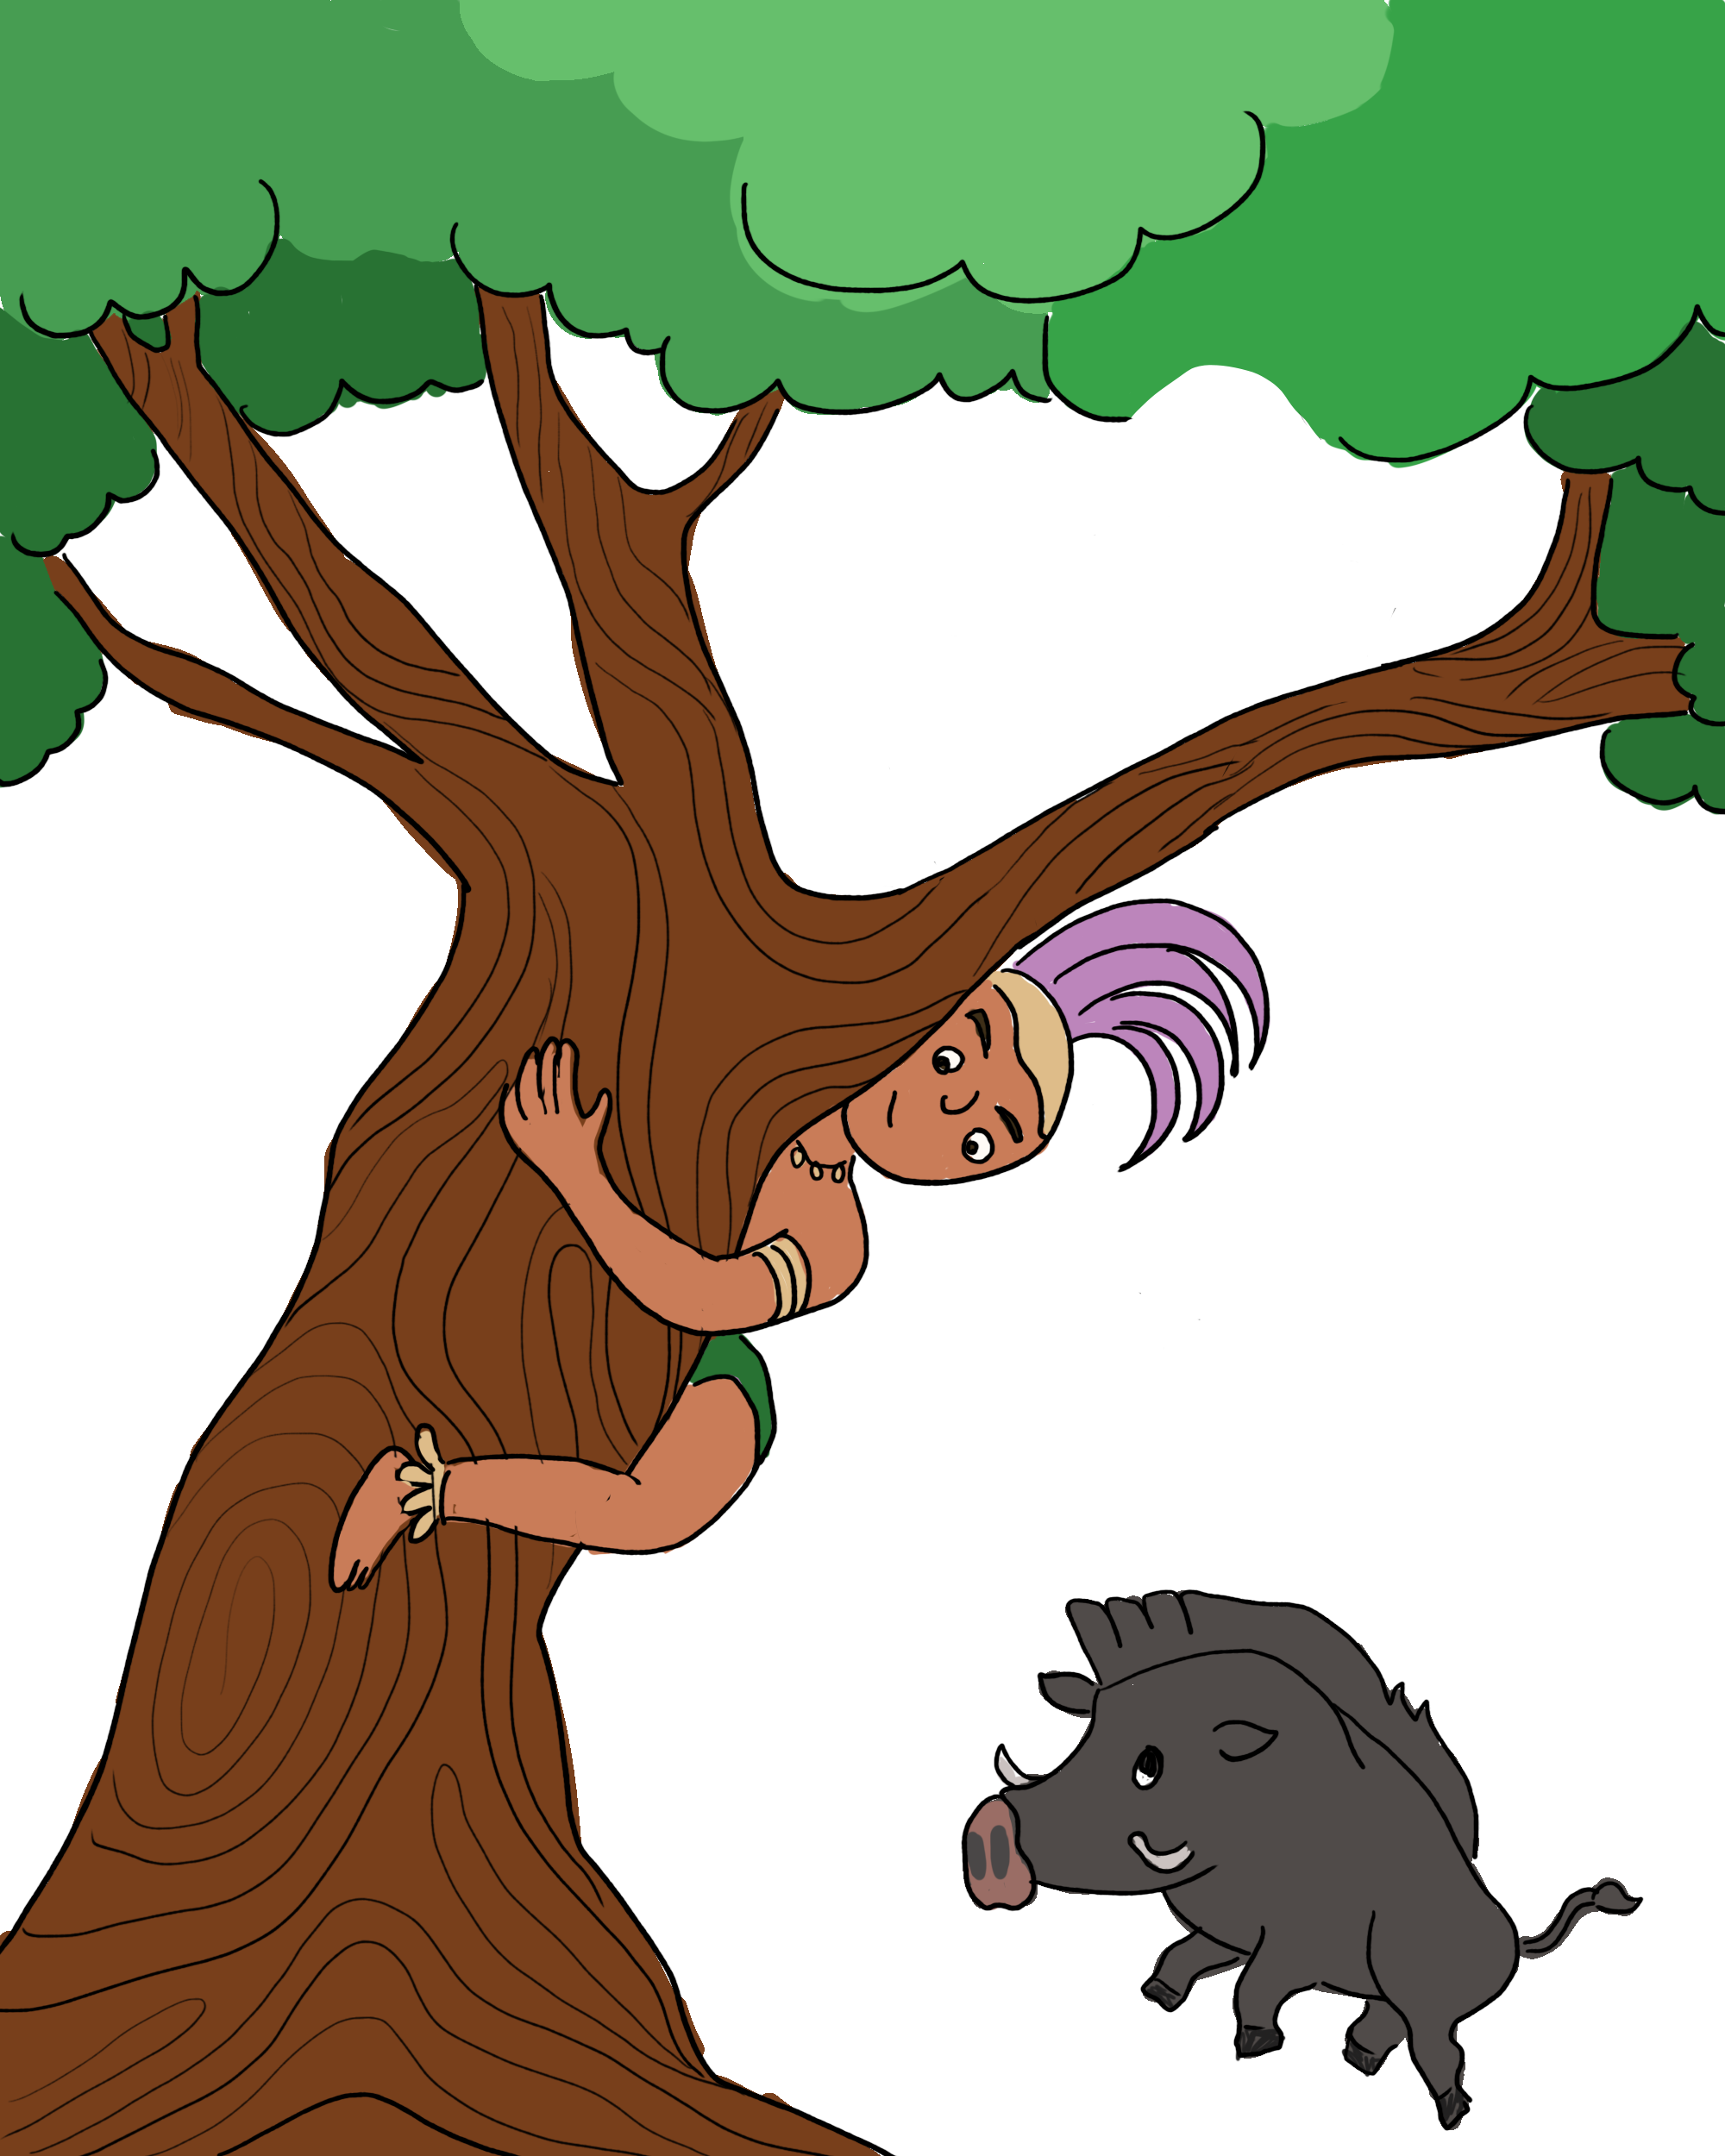
\includegraphics[width=1\linewidth]{20.12-pi.4-2}
		\vspace*{-12pt}
	\end{figure}
	\vskip 0.1cm
	\textbf{\color{toancuabi}Số Trung Hoa cổ}
	\vskip 0.1cm
	Trung Hoa cổ đại cũng là một trong những nền văn minh cổ lớn của thế giới. Khoảng $3500$ năm trước, người Trung Hoa khắc lên những mảnh mai rùa những ký hiệu khác nhau thể hiện số và chữ. Một số trong đó như~sau:
	\begin{figure}[H]
		\centering
		\vspace*{5pt}
		\captionsetup{labelformat= empty, justification=centering}
		\includegraphics[height=0.8\linewidth]{china1}\quad
		\includegraphics[height=0.8\linewidth]{41}
		\caption{\textit{\color{toancuabi}Một số ký hiệu viết trên một mảnh mai rùa.}}
		\vspace*{-10pt}
	\end{figure}
	Cách ghi số Trung Hoa cổ tương tự như cách ghi số La Mã: các chữ số giá trị lớn hơn được đặt bên trái các chữ số có  giá trị nhỏ hơn, số được biểu diễn có giá trị bằng tổng các chữ số trong biểu diễn của nó. Ví dụ \includegraphics[scale=0.25]{china5} biểu diễn số $500 + 30 + 5 = 535$. Những biểu tượng khắc trên những mảnh mai rùa phát triển theo thời gian và hình thành nên chữ viết của người Trung Hoa ngày nay. 
	\begin{figure}[H]
		\centering
		\vspace*{-5pt}
		\captionsetup{labelformat= empty, justification=centering}
		\includegraphics[width=0.9\linewidth]{20.12-pi.3}
		\vspace*{-10pt}
	\end{figure}
	Các em có thấy rằng cách biểu diễn số của người Ai Cập, La Mã và Trung Hoa cổ có điểm tương đồng? Người ta nói đó là những hệ thống số ``\textit{đơn phân}". Mỗi ký hiệu thể hiện một giá trị không thay đổi cho dù nó đứng ở vị trí nào. Mỗi số viết ra biểu diễn một đại lượng được xác định bằng cách  cộng (hay trừ như ở số La Mã) những giá trị tương ứng với các ký hiệu được sử dụng trong đó. Số mà chúng ta dùng ngày nay là một hệ thống số ``\textit{sắp theo hàng}" vì các ký hiệu có giá trị phụ thuộc vào hàng mà nó được xếp vào. Ở hàng chục, số $1$ có nghĩa là một chục, nhưng số $1$ ở hàng đơn vị có nghĩa là $1$ đơn vị. Trong khi đó, số của người Babylon và người Maya là một dạng hỗn hợp vừa được ``\textit{sắp theo hàng}" vừa cần cộng những ký hiệu trong mỗi hàng để biết giá trị của số được biểu diễn.
	\vskip 0.1cm
	Vậy là qua bài viết này chúng ta đã biết những cách ghi số  từ thời xa xưa của con người ở những nơi khác nhau trên Trái Đất. Những đại lượng phức tạp hơn, như phân số chẳng hạn, cũng đã được người cổ đại viết ra và sử dụng. Chúng ta sẽ tìm hiểu thêm về những thành tựu toán học của loài người ở những thời kỳ trước đây trong những số báo sắp tới nhé. 
	\vskip 0.1cm
	\textbf{\color{toancuabi}Bài tập} $\pmb{1.}$
	Em viết các số sau theo cách viết số ngày nay
	\vskip 0.1cm
	$\bullet$ \includegraphics[scale=0.5]{babylon1}
	\vskip 0.1cm
	$\bullet$ \includegraphics[scale=0.42]{babylon2}
	\vskip 0.1cm
	$\bullet$ \includegraphics[scale=0.42]{maya1}
	\vskip 0.1cm
	$\bullet$ \includegraphics[scale=0.42]{maya2}
	\vskip 0.1cm
	$\bullet$ \includegraphics[scale=0.5]{china2}
	\vskip 0.1cm
	$\bullet$ \includegraphics[scale=0.5]{china4}
	\vskip 0.1cm
	\textbf{\color{toancuabi}Bài tập} $\pmb{2.}$ Em hãy viết số $2022$ theo cách ghi số Babylon, Maya và Trung Hoa cổ.
	\vskip 0.1cm
	\textbf{\color{toancuabi}Tài liệu, nguồn tham khảo}
	\vskip 0.1cm
	[$1$] R. L. Cooke, History of math, Wiley, $2013$.
	\vskip 0.1cm
	[$2$] \url{https://www.britannica.com/}
	\vskip 0.1cm
	[$3$] \url{https://www.penn.museum/}
	\vskip 0.1cm
	[$4$] \url{https://www.cemc.uwaterloo.ca}
\end{multicols}
\newpage
\graphicspath{{../toancuabi/pic/}}
\begingroup
\AddToShipoutPicture*{\put(150,680){\includegraphics[scale=1]{../tieude.pdf}}} 
\centering
\endgroup
\vspace*{25pt}

\begin{multicols}{2}
	Trong giờ nghỉ trưa, thám tử Xuân Phong vẫn đang ngồi miệt mài đọc các tài liệu điều tra phá án, thì bỗng ``choang", một tiếng vỡ chói tai vang lên từ phía cửa sổ. Ngẩng lên, Xuân Phong nhìn thấy bốn cậu thiếu niên chạy thục mạng về phía cuối phố. Chắc hẳn lại là một trò nghịch tinh quái nào đó rồi.
	\vskip 0.15cm 
	Xuân Phong nhờ phía cảnh sát đưa bốn cậu thiếu niên nghịch ngợm này vào trụ sở để thẩm vấn. Bốn cậu lần lượt tên là An, Vinh, Sinh và Du. An tuyên bố ``Vinh là người làm vỡ kính", Vinh lại khẳng định ``Sinh là người có lỗi",  Sinh thì quả quyết ``Vinh nói dối đấy", còn Du thề rằng ``Cháu không làm điều này". 
	Sau một hồi nói chuyện, Xuân Phong mới biết rằng chỉ có duy nhất một cậu  trong số họ là nói thật. Vậy ai là người làm vỡ kính phòng làm việc của thám tử Xuân Phong nhỉ?
	\begin{figure}[H]
		\vspace*{-5pt}
		\centering
		\captionsetup{labelformat= empty, justification=centering}
		\includegraphics[width= 1\linewidth]{xp}
		\vspace*{-12pt}
	\end{figure}
\end{multicols}
\vspace*{-10pt}
\rule{1\linewidth}{0.1pt}
\begingroup
\AddToShipoutPicture*{\put(112,380){\includegraphics[scale=1]{../tieude11.pdf}}} 
\centering
\endgroup
\vspace*{46pt}

\begin{multicols}{2}
	$\pmb{1.}$ Có $30$ bạn học sinh tham gia một cuộc thi hùng biện bằng tiếng Anh. Các bạn lần lượt chọn các câu hỏi và trả lời theo thứ tự xếp hàng. Bạn thứ nhất được $80$ điểm, bạn thứ hai được $60$ điểm, bạn thứ ba có số điểm bằng trung bình cộng của bạn thứ nhất và bạn thứ hai, bạn thứ tư có số điểm bằng trung bình cộng của ba bạn đầu tiên. Nói chung, kể từ bạn thứ ba trở đi thì  mỗi một bạn học sinh tiếp theo luôn có số điểm bằng trung bình cộng số điểm của các bạn đã thi trước đó. 
	\begin{figure}[H]
		\centering
		\vspace*{-5pt}
		\captionsetup{labelformat= empty, justification=centering}
		\includegraphics[width=0.92\linewidth]{bai1}
%		\vspace*{-5pt}
	\end{figure}
	Hỏi bạn cuối cùng, tức bạn có số thứ tự $30$, đạt được bao nhiêu điểm trong cuộc thi? 
	\vskip 0.1cm
	$\pmb{2.}$ Vào một ngày hè, ba bạn Yến, Vinh và Công đến hiệu kem và mỗi bạn đều lấy đủ $3$ vị: trái cây, vani và sô--cô--la (mỗi vị một cốc). Sau khi ăn xong, vì $3$ cốc cho một người là chưa đủ, nên Yến lấy thêm một cốc kem trái cây, Vinh lấy thêm một cốc kem vani và Công lấy thêm một cốc kem sô--cô--la. 
	\begin{figure}[H]
		\centering
		\vspace*{-5pt}
		\captionsetup{labelformat= empty, justification=centering}
		\includegraphics[width=0.9\linewidth]{bai2}
		\vspace*{-5pt}
	\end{figure}
	Lúc ra quầy thanh toán, Yến phải trả $70$ nghìn, Vinh phải trả $80$ nghìn còn Công phải trả $90$ nghìn. Hỏi mỗi vị kem có giá bao nhiêu tiền một cốc?
	\vskip 0.1cm
	$\pmb{3.}$ Ba chú khỉ con dễ thương có tên là Bibi, Bobo, và Bubu được diện áo và giày thật đẹp để quay video đăng YouTube. Các chú được mặc ba chiếc áo có các màu khác nhau là đỏ, xanh lá cây và xanh lơ. Giày của ba chú cũng có ba màu như thế, mỗi chú mang một màu. Bibi thì diện áo và giày có cùng màu. Bobo lại không thích màu đỏ, nên cả giày và áo đều không phải đỏ. Bubu thì mang giày xanh lá cây, còn áo lại khác màu giày. Vậy các chú khỉ đã mặc áo và đi giày có màu như thế nào nhỉ?
	\begin{figure}[H]
		\centering
		\vspace*{-5pt}
		\captionsetup{labelformat= empty, justification=centering}
		\includegraphics[width=1\linewidth]{bai3}
		\vspace*{-15pt}
	\end{figure}
	$\pmb{4.}$ Để chuẩn bị cho cuộc đua xe đạp sắp diễn ra, sáng sớm Gấu con đã mang xe ra tập luyện. Lúc đi tốc độ của Gấu con là $15$ dặm/giờ. Do đường khá đông nên chiều trở về dù vẫn đi trên con đường đó nhưng Gấu con chỉ di chuyển với tốc độ $10$ dặm/giờ. Hỏi trên cả quãng đường lúc đi và về vận tốc trung bình của Gấu con là bao nhiêu?
	\begin{figure}[H]
		\centering
		\vspace*{-5pt}
		\captionsetup{labelformat= empty, justification=centering}
		\includegraphics[width=1\linewidth]{bai4}
		\vspace*{-5pt}
	\end{figure}
	$\pmb{5.}$ Trên bàn có một đống đá cuội gồm $1001$ viên. Người ta lấy ra một viên đá và chia đống đá ra  thành hai đống mới, sao cho mỗi đống có ít nhất $3$ viên. Bây giờ, trong mỗi một đống đá mới, người ta lại lấy ra một viên đá và chia đống đó ra thành hai đống mới, và cứ tiếp tục như vậy. Hỏi có thể lấy các viên đá sao cho sau một số lần lấy, trên bàn chỉ còn toàn các đống đá mà mỗi đống có đúng $3$ viên được hay không?
	\begin{figure}[H]
		\centering
		\vspace*{-5pt}
		\captionsetup{labelformat= empty, justification=centering}
		\includegraphics[width=1\linewidth]{bai5}
		\vspace*{-15pt}
	\end{figure}
	$\pmb{6.}$ Thạch Sanh chuẩn bị lên đường tiêu diệt Mãng xà -- con quái vật có tận $3$ cái đầu và $3$ cái đuôi gớm ghiếc. Ngài Thần Miếu đưa cho chàng một bảo bối và dặn dò: ``Đây là chiếc gươm thần thiêng liêng. Bằng một nhát gươm, con có thể chém đứt được một cái đầu, hoặc là hai cái đầu, hoặc là một cái đuôi, hoặc là hai cái đuôi của con Mãng xà. Nhưng con nên nhớ, nếu con chỉ chém đứt một cái đầu, thì một cái đầu khác của nó sẽ mọc lên, nếu chỉ chém đứt một cái đuôi, thì hai cái đuôi khác lại mọc ra, nếu chém đứt hai cái đuôi thì một cái đầu khác lại mọc ra, còn nếu con chém đứt được hai cái đầu thì không có gì mọc ra thêm nữa". Vậy Thạch Sanh có thể chém đứt tất cả đầu và đuôi của con Mãng xà sau bao nhiêu nhát gươm?
	\begin{figure}[H]
		\centering
		\vspace*{-5pt}
		\captionsetup{labelformat= empty, justification=centering}
		\includegraphics[width=1\linewidth]{bai6}
		\vspace*{-5pt}
	\end{figure}
\end{multicols}
\newpage
\begingroup
\AddToShipoutPicture*{\put(112,640){\includegraphics[scale=1]{../tieude2.pdf}}} 
\centering
\endgroup
\graphicspath{{../toancuabi/pic/}}
\vspace*{65pt}

\begin{multicols}{2}
	$\pmb{1.}$ Trong một kỳ nghỉ hè, Tâm và Bảo cùng đi du lịch trên một chuyến tàu hỏa. Hai toa mà họ ngồi là các toa liền kề nhau. Toa tàu của Tâm là toa thứ $5$ tính từ đầu tàu, còn toa  của Bảo lại là toa thứ $7$ tính từ đuôi tàu. Hỏi đoàn tàu của hai bạn hôm đó có bao nhiêu toa?
	\begin{figure}[H]
		\vspace*{-5pt}
		\centering
		\captionsetup{labelformat= empty, justification=centering}
		\includegraphics[width= 1\linewidth]{b1}
		\vspace*{-15pt}
	\end{figure}
	\textit{Lời giải.} Tùy thuộc vào việc Tâm ngồi gần đầu tàu hơn Bảo hay Bảo ngồi gần đầu tàu hơn Tâm.
	\vskip 0.1cm
	Nếu Tâm ngồi gần hơn, rõ ràng số toa là $5+7=12$.
	\vskip 0.1cm
	Tuy nhiên, nếu Bảo ngồi gần đầu tàu hơn, thì số toa sẽ là $5+7-2=10$ (toa).
	\vskip 0.1cm
	Ở đây $2$ là hai toa của Tâm và Bảo.
	\vskip 0.1cm
	$\pmb{2.}$	Có ba người bạn muốn đi ca nô vượt qua một con sông, chở theo một cái tủ lạnh. Chiếc ca nô chỉ đủ chỗ cho $2$ người và tủ lạnh, hoặc chỉ cho $3$ người. Nhưng rắc rối ở chỗ là cái tủ lạnh quá nặng, nên phải có cả sức $3$ người mới đủ để khiêng nó lên ca nô hoặc đẩy xuống khỏi ca nô. Hỏi họ có thể qua được sông hay không?
	\begin{figure}[H]
		\vspace*{-10pt}
		\centering
		\captionsetup{labelformat= empty, justification=centering}
		\includegraphics[width= 1\linewidth]{b2}
		\vspace*{-15pt}
	\end{figure}
	\textit{Lời giải.} Lần đầu tiên ta cho hai bạn đi cùng chiếc tủ lạnh sang sông, một bạn sang bên kia, còn một bạn quay lại cùng chiếc tủ lạnh. Sau khi đón bạn còn lại ở bên bờ bên này, hai bạn cùng đi lần cuối cùng chiếc tủ lạnh sang nốt bên bờ bên kia, ở đó có một bạn đợi sẵn để chuyển tủ lạnh khỏi ca nô lên bờ.
	\vskip 0.1cm
	$\pmb{3.}$ Trong một vương quốc nọ các thần dân chia thành $2$ nhóm người: một nhóm Thật thà gồm toàn những người nói thật, và nhóm kia là Dối trá gồm toàn những người chỉ nói dối. Trong một buổi tối nọ, có $10$ người lần lượt bước vào một ngôi nhà, mỗi người trong số họ (trừ người cuối cùng) viết trên một mảnh giấy đặc biệt để thông báo người sẽ vào tiếp theo anh ta là Thật thà hay Dối trá. Nếu như tin vào những gì viết trên $9$ mảnh giấy đó, thì toàn là người Dối trá đã bước vào nhà. Hỏi trên thực tế có tất cả bao nhiêu người Dối trá đã tới ngôi nhà đó.	
	\begin{figure}[H]
		\vspace*{-5pt}
		\centering
		\captionsetup{labelformat= empty, justification=centering}
		\includegraphics[width= 1\linewidth]{b3}
		\vspace*{-15pt}
	\end{figure}
	\textit{Lời giải.} Mỗi một người Thật thà (trừ người đầu tiên) bước vào nhà đều phải có một người Dối trá đi trước anh ta, còn mỗi người Dối trá thì lại phải có một người Thật thà đi đằng trước. Suy ra, trong cả hai trường hợp người đầu tiên là Thật thà hay Dối trá, có tất cả $5$ người Thật thà và $5$ người Dối trá đã bước vào nhà đó.
	\vskip 0.1cm
	$\pmb{4.}$ Hai chiếc máy bơm cùng nhau bơm đầy nước cho một bể bơi trong vòng $2$ giờ. Hỏi mỗi chiếc máy bơm sẽ bơm đầy bể trong bao nhiêu lâu, biết rằng thời gian bơm đầy của hai máy bơm tính theo giờ là các số nguyên khác nhau.
	\begin{figure}[H]
		\vspace*{-5pt}
		\centering
		\captionsetup{labelformat= empty, justification=centering}
		\includegraphics[width= 0.9\linewidth]{b4}
		\vspace*{-10pt}
	\end{figure}
	\textit{Lời giải.} 	Giả sử một máy bơm đầy bể trong $a$ (giờ) còn máy kia trong $b$ (giờ). Ta có $a,b$ là các số nguyên khác nhau. Trong $1$ giờ, máy thứ nhất bơm được $\dfrac{1}{a}$ phần bể, còn máy kia bơm được $\dfrac{1}{b}$ phần bể. Theo giả thiết $\dfrac{1}{a}+\dfrac{1}{b}= \dfrac{1}{2}$.
	\vskip 0.1cm
	Rõ ràng $a,b$ phải lớn hơn $2$. Không mất tính tổng quát, giả sử $2<a<b$. 
	\vskip 0.1cm
	Nếu $a = 3$ thì ta có $b = 6$.
	\vskip 0.1cm
	Nếu $a \ge 4$, thì $b \ge 5$, và $\dfrac{1}{a} + \dfrac{1}{b} < \dfrac{1}{4} + \dfrac{1}{4} = \dfrac{1}{2}$, do đó ta loại những trường hợp này.
	\vskip 0.1cm
	Vậy một máy bơm đầy bể trong $3$ giờ và máy còn lại bơm đầy bể trong $6$ giờ.
	\vskip 0.1cm
 	$\pmb{5.}$ Trên một hòn đảo nọ có các thổ dân sinh sống, một số người thì luôn nói thật, còn những người còn lại thì luôn nói dối. Một lần nọ, ba thổ dân là anh Tit, anh Te và anh Tu gặp nhau. Một người trong số họ nói ``Tit và Te -- cả hai đều là những  người nói dối'', một người khác nói ``Tit và Tu -- cả hai đều là những người nói dối" (tuy nhiên không rõ chính xác ai nói những câu này). Hỏi có bao nhiêu người nói dối trong số ba người này?
	\begin{figure}[H]
		\vspace*{-5pt}
		\centering
		\captionsetup{labelformat= empty, justification=centering}
		\includegraphics[width= 1\linewidth]{b5}
		\vspace*{-15pt}
	\end{figure}
	\textit{Lời giải.} Có tất cả $2$ người nói dối trong số họ. Thật vậy, nếu trong số ba người trên có không quá một người nói dối, thì trong số hai câu nói trên, phải có ít nhất một câu là thật (do hai người khác nhau nói ra). Nhưng theo bất kỳ câu nào, thì số người nói dối trong họ phải ít nhất là $2$. Suy ra vô lý.
	\vskip 0.1cm
	Nếu cả ba người cùng nói dối, thì cả hai câu đều là thật, mà lại do các người nói dối phát biểu. Điều này cũng không thể.
	\vskip 0.1cm
	Vì vậy số người nói dối phải đúng bằng $2$.
	\vskip 0.1cm
	Ta còn phải đưa ra ví dụ về tình huống có thể xảy ra. Ví dụ như anh Tit là người nói thật, còn hai câu trên đều do hai anh nói dối phát ngôn.
	\vskip 0.1cm
	$\pmb{6.}$ Có $10$ cái hộp bút, mỗi hộp đựng một số chiếc bút chì màu, không có hộp nào là rỗng. Biết rằng số bút chì ở hai hộp bất kỳ là khác nhau, hơn nữa những chiếc bút chì trong mỗi hộp đều có màu khác nhau, em hãy chỉ ra là có thể nhặt ra từ mỗi chiếc hộp một chiếc bút để nhận được $10$ chiếc bút chì có màu hoàn toàn khác nhau. 
	\begin{figure}[H]
		\vspace*{-5pt}
		\centering
		\captionsetup{labelformat= empty, justification=centering}
		\includegraphics[width= 1\linewidth]{b6}
		\vspace*{-15pt}
	\end{figure}
	\textit{Lời giải.} Ta sắp xếp các hộp bút theo thứ tự tăng dần về số bút chì trong hộp. Vậy hộp thứ nhất có ít nhất $1$ chiếc, hộp thứ hai có ít nhất $2$ chiếc, v.v. và hộp thứ $10$ có ít  nhất $10$ chiếc bút.
	\vskip 0.1cm
	Trong hộp thứ nhất ta lấy $1$ chiếc bút, gọi màu của nó là $A$. Vì trong hộp thứ hai có ít nhất hai bút khác màu, nên ít nhất phải có một chiếc bút trong hộp này khác màu với $A$. Ta gọi  màu của chiếc bút này là  $B$. Trong hộp thứ ba có ít nhất $3$ chiếc bút khác màu nhau, nên phải có ít nhất một chiếc bút khác màu với $A$ và $B$. Ta lấy ra chiếc bút đó. Cứ làm liên tiếp như vậy ta có thể lấy ra ở mỗi hộp một chiếc bút theo như yêu cầu đề bài.
\end{multicols}
\newpage
\begingroup
\thispagestyle{toancuabinone}
\blfootnote{$^1$\color{toancuabi}Trường THCS Archimedes, Hà Nội.}
\AddToShipoutPicture*{\put(60,733){\includegraphics[width=17.2cm]{../mathc.pdf}}}
%\AddToShipoutPicture*{\put(-2,733){\includegraphics[width=17.2cm]{../mathl.pdf}}} 
\AddToShipoutPicture*{\put(192,675){\includegraphics[scale=1]{../tieude3.pdf}}} 
\centering
\endgroup
\graphicspath{{../toancuabi/pic/}}
\vspace*{35pt}

\begin{multicols}{2}
	\PIbox{\textbf{\color{toancuabi}Problem} $\pmb{1.}$ How many ways are there to go from $A$ to $B$ in the directions indicated by the pink arrows?}
	\begin{center}
		\begin{tikzpicture}[color=toancuabi, xscale=2.15, yscale=2.15]
			\draw (0,0) grid (2,2);
			\draw (0,2) node[left] {$A$};
			\draw (2,0) node[right] {$B$};
			\draw [-stealth] (2.5,2) --(3,2);
			\draw [-stealth] (2.5,2) --(2.9,1.6);
			\draw [-stealth] (2.5,2) --(2.5,1.5);
			\draw (0,1) --(1,0) (0,2) -- (2,0) (1,2) -- (2,1);
		\end{tikzpicture}
	\end{center}
	\PIbox{\textbf{\color{toancuabi}Rule of Sum:} Suppose that we have to do two independent jobs $A$ and $B$, and that there are $m$ ways to do job $A$ and $n$ ways to do job $B$. We cannot do both jobs at the same time, therefore there are $(m + n)$ ways to do one of the two jobs (either job $A$ or job $B$).}
	\vskip 0.1cm
	\textit{Solution:} In the picture below, the number at each node indicates how many ways we can go from $A$ to that node. 
	\begin{center}
		\begin{tikzpicture}[color=toancuabi, xscale=2.15, yscale=2.15]
			\draw (0,2) node[left] {$A$};
			\draw (0,2) node[above] {$1$};
			\draw (1,2) node[above] {$1$};
			\draw (2,2) node[above] {$1$};
			\draw (2,1) node[right] {$5$};
			\draw (0,1) node[left] {$1$};
			\draw (1,1.2) node[right] {$3$};
			\draw (2,0) node[below] {$\boxed{13}$};
			\draw (0,0) node[left] {$1$};
			\draw (1,0) node[below] {$5$};
			\draw (2,0) node[right] {$B$};
			\draw [-stealth] (2.5,2) --(3,2);
			\draw [-stealth] (2.5,2) --(2.9,1.6);
			\draw [-stealth] (2.5,2) --(2.5,1.5);
			\draw[-stealth] (0,1) --(1,0); 
			\draw[-stealth] (0,2) -- (1,1);
			\draw[-stealth] (1,1) -- (2,0);
			\draw[-stealth] (1,2) -- (2,1);
			\draw[-stealth]	(0,2) -- (0,1);
			\draw[-stealth]	(0,1) -- (0,0);
			\draw[-stealth]	(0,0) -- (1,0);
			\draw[-stealth]	(1,0) -- (2,0);
			\draw[-stealth]	(2,2) -- (2,1);
			\draw[-stealth]	(2,1) -- (2,0);
			\draw[-stealth]	(0,2) -- (1,2);
			\draw[-stealth] (1,2) -- (2,2);
			\draw[-stealth] (0,1) -- (1,1);
			\draw[-stealth]	(1,1) -- (2,1);
			\draw[-stealth]	(1,2) -- (1,1);
			\draw[-stealth] (1,1) -- (1,0);
		\end{tikzpicture}
	\end{center}
	To go from $A$ to $B$, we must pass through one of the three points which lie directly in front of $B$ in the directions of the arrows. These are the points indicated by the numbers $5$, $3$, $5$. Thus, the number of ways to go from $A$ to $B$ is given by
	\begin{align*}
		\text{Rule of Sum: } 5+3+5=13.
	\end{align*}
%	\textit{Answer:} $13$
%	\vskip 0.1cm
	\PIbox{\textbf{\color{toancuabi}Problem} $\pmb{2.}$ How many ways are there to go from $A$ to $B$ in the directions indicated by the given blue arrows?}
	\begin{center}
		\begin{tikzpicture}[color=toancuabi,,scale=1.1]
			\draw (0,0) rectangle (3,3);
			\draw (0,0) node[left] {$A$};
			\draw (4,4) node[right] {$B$};
			\draw[dashed] (0,0) -- (1,1) (1,1) --(4,1) (1,1) --(1,4);
			\draw (1,4) -- (4,4) (4,4) -- (3,3) (4,4) -- (4,1) (4,1) -- (3,0) (1,4) -- (0,3); 
			\draw [quantoan,-stealth] (5,1) --(5,2);
			\draw [quantoan,-stealth] (5,1) --(5.8,1.8);
			\draw [quantoan,-stealth] (5,1) --(6,1);
		\end{tikzpicture}
	\end{center}
	\textit{Solution:} 
	Using the same argument as in Problem $1$, we have:
	\begin{align*}
		\text{Rule of Sum: } 2+2+2=6.
	\end{align*}
	\begin{center}
		\begin{tikzpicture}[color=toancuabi,scale=1.1]
			\draw (0,0) rectangle (3,3);
			\draw (0,0) node[left] {$A$};
			\draw (4,4) node[above] {$B$};
			
			\draw (1,1) node[left] {$1$};
			\draw (4,4) node[right] {$6$};
			\draw (3,3) node[above] {$2$};
			\draw (3.1,0) node[right] {$1$};
			\draw (1,4) node[above] {$2$};
			\draw (4,1) node[right] {$2$};
			\draw[dashed] (0,0) -- (1,1) (1,1) --(4,1) (1,1) --(1,4);
			\draw (1,4) -- (4,4) (4,4) -- (3,3) (4,4) -- (4,1) (4,1) -- (3,0) (1,4) -- (0,3); 
			\draw [quantoan,-stealth] (5,1) --(5,2);
			\draw [quantoan,-stealth] (5,1) --(5.8,1.8);
			\draw [quantoan,-stealth] (5,1) --(6,1);
		\end{tikzpicture}
	\end{center}
%	\textit{Answer:} $6$
%	\vskip 0.1cm
	\PIbox{\textbf{\color{toancuabi}Problem} $\pmb{3.}$ How many different moves can a knight on an $8\times8$ chessboard make?}
	\vskip 0.05cm
	\textit{Problem analysis:} A knight can go from any of the $64$ squares on a chessboard.
	\vskip 0.1cm
	$\circ$ If the knight stands on a corner square, it has two possible moves.
	\vskip 0.1cm
	$\circ$ If the knight stands on a side square next to a corner square, it has three possible moves.
	\vskip 0.1cm
	$\circ$ If the knight stands on another side square, it has four possible moves, and so on.
	\vskip 0.1cm
	$\circ$ The maximum number of moves for a knight is eight when it stands on a square where it can move in all possible directions.
	\vskip 0.1cm
	The table below shows the number of moves a knight can make from each square on the board:
	\begin{center}
		\def\myNotes{{{2,3,4,4,4,4,3,2},{3,4,6,6,6,6,4,3},{4,6,8,8,8,8,6,4},{4,6,8,8,8,8,6,4},{4,6,8,8,8,8,6,4},{4,6,8,8,8,8,6,4},{3,4,6,6,6,6,4,3},{2,3,4,4,4,4,3,2}}} 
		\begin{tikzpicture}[scale=0.88,color=cackithi]
			\foreach \x  in {1,2,...,8}
			\foreach \y in {1,2,...,8}
			{	
				\draw (\x,\y*-1) +(-.5,-.5) rectangle ++(.5,.5);
				\begin{scope}[shift={(\x,\y*-1)}]
					\pgfmathtruncatemacro{\r}{\myNotes[\y-1][\x-1]}
					\coordinate (C) at (0,0,0);
					\node (C) {$\r$};
				\end{scope}
			}
		\end{tikzpicture}
	\end{center}
	Thus, the total number of moves that the knight can make on an $8\times8$ chessboard is: 
	\begin{align*}
		&\text{Rule of Sum: }\\
		&2\times4 \!+\! 3\!\times\!8 \!+\! 4\!\times\!20 \!+\! 6\!\times\!16 \!+\! 8\!\times\!16 \!=\! 336.
	\end{align*}
%	\textit{Answer:} $336$.
%	\vskip 0.1cm
	\PIbox{\textbf{\color{toancuabi}Exercise} $\pmb{1.}$ How many ways are there to go from $A$ to $B$ in the directions indicated by the pink arrows?}
	\begin{center}
		\begin{tikzpicture}[color=cackithi,scale=1.1]
			\draw  (0.,0.)-- (5.,0.);
			\draw  (5.,0.)-- (2.5,4.330127018922194);
			\draw  (2.5,4.330127018922194)-- (0.,0.);
			\draw  (2.,3.464101615137755)-- (3.,3.4641016151377553);
			\draw  (1.5,2.598076211353316)-- (3.5,2.5980762113533165);
			\draw  (1.,1.7320508075688774)-- (4.,1.732050807568878);
			\draw  (0.5,0.8660254037844387)-- (4.5,0.8660254037844392);
			\draw  (1.,0.)-- (3.,3.4641016151377553);
			\draw  (3.5,2.5980762113533165)-- (2.,0.);
			\draw  (4.,1.732050807568878)-- (3.,0.);
			\draw  (4.5,0.8660254037844392)-- (4.,0.);
			\draw  (4.,0.)-- (2.,3.464101615137755);
			\draw  (1.5,2.598076211353316)-- (3.,0.);
			\draw  (2.,0.)-- (1.,1.7320508075688774);
			\draw[-stealth,toancuabi]  (4.,4.)-- (4.5,4.86602540378444);
			\draw[-stealth,toancuabi]  (4.,4.)-- (5.,4.);
			\draw[-stealth,toancuabi]  (4.,4.)-- (4.5,3.133974596215561);
			\draw  (1.,0.)-- (0.5,0.8660254037844387);
		

			\draw (-0.3328996275042767,0.139482532970907) node {$A$};

			\draw (5.354808013691732,0.139482532970907) node {$B$};
		
		\end{tikzpicture}
	\end{center}
	\PIbox{\textbf{\color{toancuabi}Exercise} $\pmb{2.}$ A bug walks along the lines on the grid in the directions indicated by the blue arrows.  In how many ways can it get from $A$ to $B$?}
	\begin{center}
		\begin{tikzpicture}[xscale=1.95, yscale=1.95, toancuabi]
			\draw (0,0) grid (2,2);
			\draw[dashed] (0.6,0.6) -- (0.6, 2.6)  (2.6,0.6) -- (0.6,0.6) (0.3,0.3) -- (0.3, 2.3)  (2.3,0.3) -- (0.3,0.3) (0,0) -- (0.6,0.6);
			\draw (0.6,2.6) -- (2.6,2.6) (2.6,2.6) -- (2.6,0.6) (0.3,2.3) -- (2.3,2.3) (2.3,2.3) -- (2.3,0.3);
			\draw (0,2) -- (0.6, 2.6) (1,2) -- (1.6, 2.6) (2,2) -- (2.6,2.6) (2,1) --(2.6,1.6) (2,0) -- (2.6,0.6);
			\draw[dashed] (1,0) -- (1.6, 0.6) (1.6, 0.6) -- (1.6,2.6) (0,1) -- (0.6,1.6) (0.6,1.6) -- (2.6,1.6) (1,1) -- (1.6,1.6) (1.3,2.3) -- (1.3,0.3) (0.3,1.3) -- (2.3,1.3);
			\draw[quantoan,-stealth] (3,0.6) -- (3,1.1);
			\draw[quantoan,-stealth] (3,0.6) -- (3.5,0.6);
			\draw[quantoan,-stealth] (3,0.6) -- (3.4,1);
			\draw (0,0) node[left] {$A$};
			\draw (2.6,2.6) node[right] {$B$};
 		\end{tikzpicture}
	\end{center}
	\PIbox{\textbf{\color{toancuabi}Exercise} $\pmb{3.}$ How many different moves can a bishop on an $8\times8$ chessboard make?}
	\vskip 0.2cm
	\PIbox{
	\textbf{\color{toancuabi}\color{toancuabi}New words}
	\vskip 0.1cm
	{\color{toancuabi}arrow:} mũi tên
	\vskip 0.1cm
	{\color{toancuabi}move:} nước đi 
	\vskip 0.1cm
	{\color{toancuabi}node:} điểm nút (lưới)
	\vskip 0.1cm
	{\color{toancuabi}knight:} quân mã
	\vskip 0.1cm
	{\color{toancuabi}bishop:} quân tượng
	\vskip 0.1cm
	{\color{toancuabi}bug:} con bọ}
\end{multicols}